\documentclass{article}
\usepackage[utf8x]{inputenc}
\usepackage{polski}
\usepackage{pythonhighlight}

\usepackage{amssymb, amsmath, amsfonts, amsthm, cite, mathtools, enumerate, rotating, hyperref,soul}
\newcommand \eq[1]{\begin{equation} \begin{split}  #1 \end{split} \end{equation}}


\makeatletter
\newcommand\tab[1][1cm]{\hspace*{#1}}
\def\@seccntformat#1{%
  \expandafter\ifx\csname c@#1\endcsname\c@section\else
  \csname the#1\endcsname\quad
  \fi}
\makeatother

\newtheorem{lemma}{Lemat}
\newtheorem{theorem}{Twierdzenie}

\title{AiSD L2Z7}
\date{31.03.2021}
\author{Maurycy Borkowski}
\begin{document}
\maketitle

\section{Zadanie 7}
Podzielmy zbiór zadań na: $S_1 = \{i: A_i < B_i\}$ i $S_2 = \{i: A_i \geq B_i\}$.\\ Posortujmy $S_1$ rosnąco po $A_i$ a $S_2$ malejąco o $B_i$. Odpowiedź $S_1 \cup S_2$.
\begin{proof}
Weźmy dowolne rozwiązanie optymalne $S$ jeżeli $S$ nie jest \textit{powyższej} postaci to musi być spełniony jeden z przypadków dla dwóch kolejnych zadań $i,j$ w $S$.\\\textbf{Możemy iterować się po kolei od $1$ do $n-1$ i sprawdzać czy każda para kolejnych zadań spełnia warunek konieczny bycia w rozwiązaniu algorytmu (poprawna kolejność w $S_{1,2}$ i poprawna kolejność procesowania najpierw $S_1$ potem $S_2$). Taka para nie znajdzie się w tym rozwiązaniu tylko wtedy gdy spełniony jeden z poniższych warunków. Jeżeli nie znajdziemy, żadnej takiej pary dla kolejnych zadań to $S$ jest powyższej postaci.}:
\begin{enumerate}
    \item $j \in S_2 \land i \in S_1$
    \item $i,j \in S_1 \land A_j > A_i$
    \item $i,j \in S_2 \land B_j < B_i$
\end{enumerate}
Pokażemy, że w każdym z tych przypadków zmiana zadań $i,j$ da nam rozwiązanie niegorsze niż $S$. Oznaczenia:\\
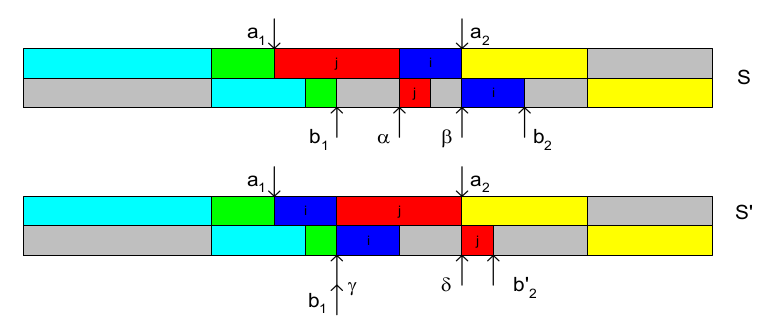
\includegraphics[scale=0.5]{zad7}
$S^\prime$ - $S$ z zamienionymi zadaniami $i,j$\\
$b_{1}$ - zakończenie poprzedniego (przed $i$) zadania w $S$\\
$b_{1}^\prime$ - zakończenie poprzedniego (przed $j$) zadania w $S^\prime$\\
$b_{2}$ - zakończenie obu zadań w $S$\\
$b_{2}^\prime$ - zakończenie obu zadań w $S^\prime$\\\\
$\alpha = \max(b_1, (A_j + a_1))$ rozpoczęcie pierwszego zadania $b$ w $S$\\
$\beta = \max(a_2, (B_j + \alpha))$ rozpoczęcie drugiego zadania $b$ w $S$\\
$b_2 = B_i + \beta = \max(a_1+A_j+A_i+B_i, B_j + B_i +b_1, B_j+B_i +A_j+a_1)$\\
$\gamma = \max(b_1,(A_i+a_1))$ rozpoczęcie pierwszego zadania $b$ w $S^\prime$\\
$\delta = \max(a_2,(B_i+\gamma))$ rozpoczęcie drugiego zadania $b$ w $S^\prime$\\
$b_2^\prime = B_j + \delta = \max(a_1+A_j+A_i+B_j, B_j + B_i +b_1, B_j+B_i +A_i+a_1)$\\
\begin{enumerate}
    \item $j \in S_2 \land i \in S_1 \implies A_j \geq B_j \land A_i < B_i$:
    $$
    \overbrace{a_1 + A_j + A_i + B_i}^{1. \quad w \quad b_2} \geq \underbrace{B_i + B_j + A_i + a_1}_{3. \quad w \quad b_2^\prime}
    $$
    $$
    \overbrace{B_j + B_i + A_j + a_1}^{3. \quad w \quad b_2} \geq \underbrace{a_1 + A_j + A_i + B_j}_{1. \quad w \quad b_2^\prime}
    $$
    \item $i,j \in S_1 \land A_j > A_i \implies A_j > A_i \land A_i < B_i$
    $$
    \overbrace{B_j + B_i + A_j + a_1}^{3. \quad w \quad b_2} > \underbrace{B_i + B_j + A_i + a_1}_{3. \quad w \quad b_2^\prime}
    $$
    $$
    \overbrace{B_j + B_i + A_j + a_1}^{3. \quad w \quad b_2} > \underbrace{a_1 + A_j + A_i + B_j}_{1. \quad w \quad b_2^\prime}
    $$
    \item $i,j \in S_2 \land B_j < B_i \implies A_j \geq B_j \land B_j < B_i$
    $$
    \overbrace{a_1 + A_j + A_i + B_i}^{1. \quad w \quad b_2} \geq \underbrace{B_i + B_j + A_i + a_1}_{3. \quad w \quad b_2^\prime}
    $$
    $$
    \overbrace{a_1 + A_j + A_i + B_i}^{1. \quad w \quad b_2} > \underbrace{a_1 + A_j + A_i + B_j}_{1. \quad w \quad b_2^\prime}
    $$
\end{enumerate}
W każdym przypadku mamy: $b_2 \geq b_2^\prime$. Zmiana nie pogarsza rozwiązania.
\end{proof}
\href{https://personal.utdallas.edu/~chandra/documents/6363/lec7.pdf}{źródło}
\clearpage
\end{document}